\documentclass[12pt]{article}
\usepackage[utf8]{inputenc}
\usepackage[margin=1in,bottom=1.5in,a4paper]{geometry}
\usepackage{tikz}
\usepackage{amsmath}
\usepackage{amssymb}
\usepackage{multicol}
\usepackage{xcolor}
\usepackage{tabularx}
\usepackage{mathtools}
\usepackage{ textcomp }
\usepackage{graphicx}
\usepackage{ stmaryrd }
\usepackage{hyperref}
\usepackage{ marvosym }
\usepackage{ dsfont }
\usepackage{ulem}
\tolerance=1000
\usepackage{fancyhdr}
\pagestyle{fancy}
\headheight 50pt

\renewcommand{\thesection}{\Alph{section}}

%edit header and footer
\fancypagestyle{firstpage}{
  \lhead{X-as-a-Service cloud assets}
  \chead{\textbf{\Large Learnings}}
  \rhead{CySec Project '21}
}
\lhead{}
\rhead{X-as-a-Service cloud assets}

\cfoot{}
\rfoot{\small\thepage}

\begin{document}
\thispagestyle{firstpage}

\section*{Cloud Services}
\begin{itemize}
    \item \textbf{IaaS: Infrastructure as a Service} \\
    Users manage applications, data, operating system, middleware and runtimes. \\
    Provider is responsible for providing virtualization, storage, network and servers. \\
    \textit{Examples: AWS EC2, Rackspace, Google Compute Engine (GCE), Digital Ocean, Magento 1 Enterprise Edition, also Azure}
    
    \item \textbf{PaaS: Platform as a Service} \\
    Often used by: developers and programmers who have ideas for an app and can also program them, but do not have the infrastructure to operate and maintain it. \\
    \textit{Examples: AWS Elastic Beanstalk, Heroku, Microsoft Azure (mostly used as PaaS), Force.com, OpenShift, Apache Stratos, Magento Commerce Cloud}
    
    \item \textbf{SaaS: Software as a Service} \\
    Users interact with the software via a web browser. \\
    \textit{Examples: BigCommerce, Google Apps, Salesforce, Dropbox, MailChimp, ZenDesk, DocuSign, Slack, Hubspot, Paychex HR-Software, CA Technology Enterprise software, WordPress Content Management Software, Microsoft Office 365}
\end{itemize}

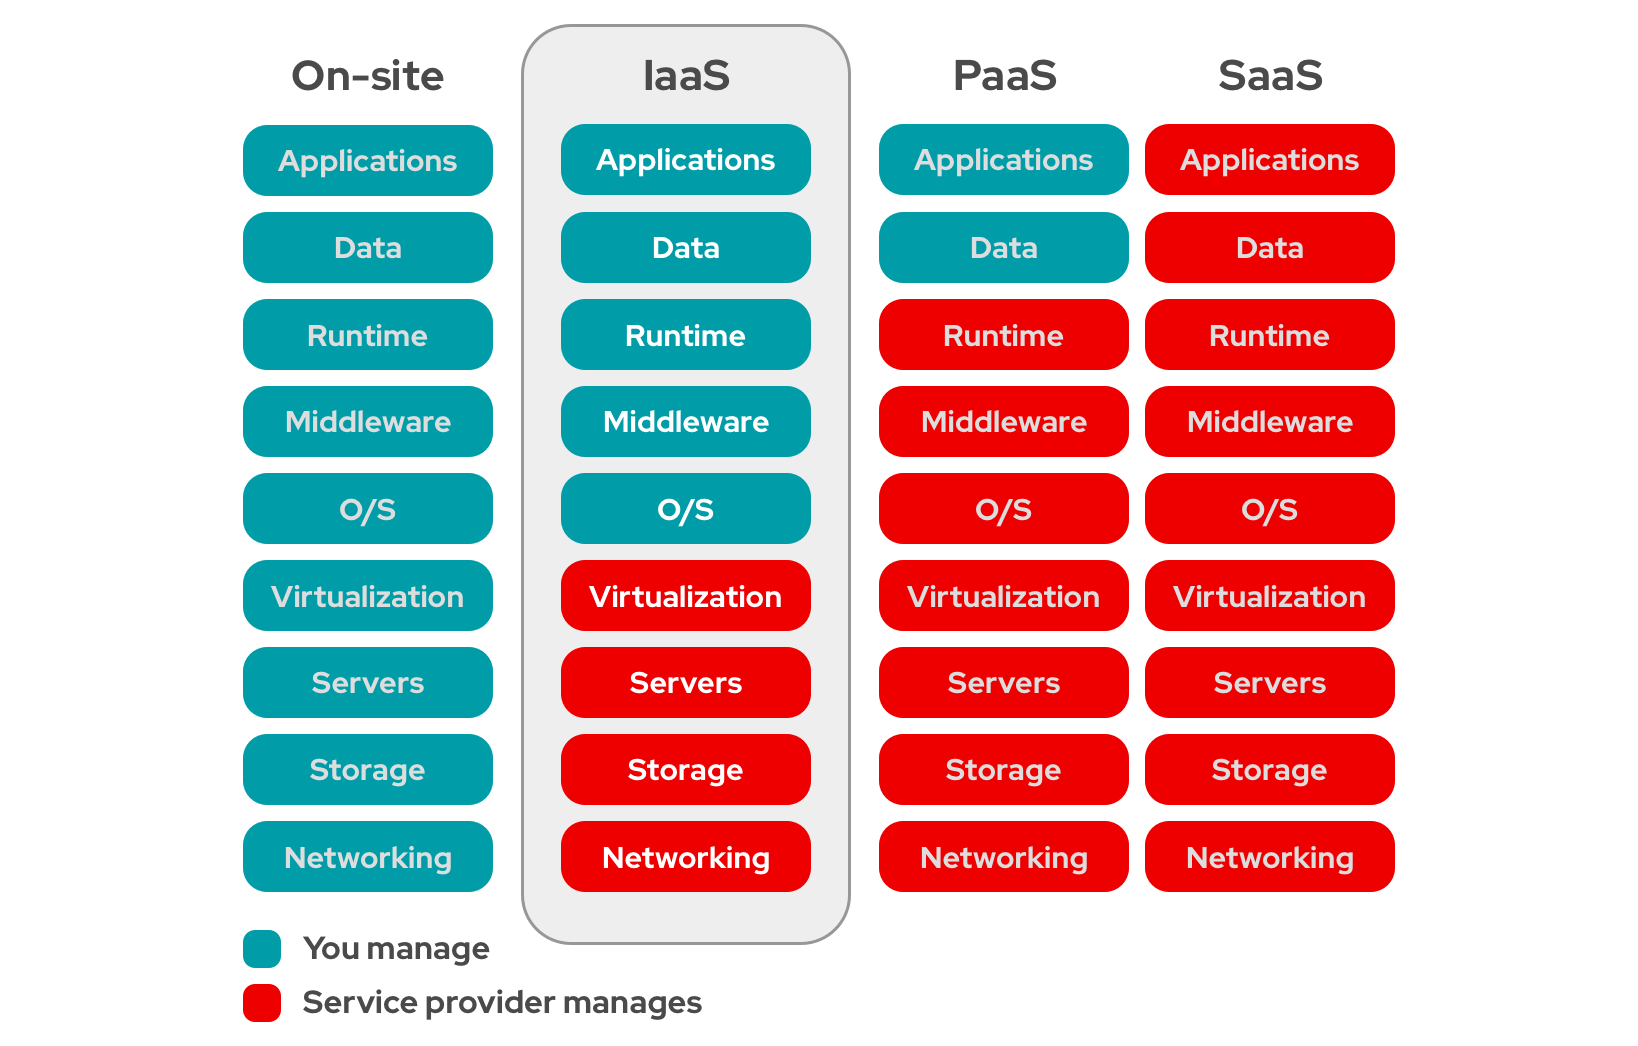
\includegraphics[scale=0.3]{as-a-Service_comparison.png}

\begin{center}
    \url{www.redhat.com/de/topics/cloud-computing/what-is-iaas}
\end{center}
"Most businesses use a combination of SaaS and IaaS cloud computing service models." \\
Also services like Security-as-a-Service (SaaS), Firewall-as-a-Service (FWaaS) or Software Infrastructure-as-a-Service (SIaaS) exist.

\section*{Cloud Providers} 
\textbf{Biggest Players} \hspace{11cm} \href{https://www.zdnet.com/article/the-top-cloud-providers-of-2021-aws-microsoft-azure-google-cloud-hybrid-saas/}{\textit{Source}}
\begin{enumerate}
    \item Amazon Web Services (AWS)
    \item Microsoft Azure
    \item Google Cloud and Anthos
    \item Alibaba Cloud (mainly China)
    \item IBM Cloud
    \item VMware (Dell)
\end{enumerate}
\textbf{Further Cloud Providers:}
\begin{itemize}
    \item Salesforce (leading in SaaS)
    \item Oracle Cloud
    \item SAP Business Technology Platform (SAP BTP) \\
    (at least SAP HANA cloud is AWS)
    \item ServiceNow
    \item Microsoft Office 365
    \item OpenStack
    \item Kamatera
    \item Adobe (at least partially AWS!)
\end{itemize}


\newpage
\section*{Misc}
\begin{itemize}
    \item Cloud-Enabler: primarily IT firms that develop hardware, software, storage, networking and other related products, serving as a cloud environment component.
    \item Cloud-Service-Provicer (CSP): vendors which provide Information Technology (IT) as a service over the Internet.
    \item Identify where a server is located: \url{https://research.domaintools.com/}
\end{itemize}
Everything that could be interesting in the future... 
\begin{itemize}
    \item ... to potentially identify which cloud service is used:
    \begin{itemize}
    \item Google Cloud offers \href{https://cloud.google.com/interconnect/docs/concepts/dedicated-overview}{\textit{Dedicated Interconnect}}
    \item AWS offers \href{https://aws.amazon.com/directconnect/}{\textit{Direct Connect}}
    \item Azure offers \href{https://azure.microsoft.com/en-us/services/expressroute/}{\textit{ExpressRoute}}
    \item OpenStack offers \href{https://www.openstack.org/passport/}{\textit{OpenStack Public Cloud Passport}}
\end{itemize}
\end{itemize}


\subsection*{Researching \& ideas}
\begin{itemize}
    \item googleapi in content security policy $\rightarrow$ using google cloud services? \\
    $\Rightarrow$ No, googleapis aren't cloud services!
    
    How about learning something out of the CSP?
    
    \item DNS entries? DNS Resolver from AWS? or CloudFront servers? Amazon Route 53 (DNS Management Service)?
    
    \item Fiddler, Wireshark, analyzing traffic?
    
    \item included scripts?
    
    \item response headers?
    
    \item certificates?
    
    \item cookies? (probably not)
\end{itemize}


\newpage
\subsection*{Understanding AWS}
\begin{itemize}
    \item Identify if website uses AWS:
    
    "Amazon has 26 different web services. You can tell if the web server you are communicating with is hosted by Amazon EC2 by its IP address. You can't tell if there are EC2 instances behind a proxy you're talking to, though.

    You can tell if the domain name is resolved by an Amazon Route 53 DNS server.

    Besides that, you wouldn't really know what other services are being used unless they choose to make it obvious."
    
    \item EC2:
    
    Elastic Compute Cloud, IaaS (and SaaS); provides scalable computing capacity in the Amazon Web Services (AWS) Cloud
    
    \item S3:
    
    Simple Storage Service; really good for static websites (html, css, js) but doesn't support server-side scripting languages (php,...)
    
    You can easily host a website via S3 bucket options. If you want your own domain name you have to register it and use Route 53: on resolution there are awsdns entries (e.g. ns-183.awsdns-22.com. / s3-website)
    
    \item AWS Certificate Manager (ACM) is a private CA service.
    
\end{itemize}

\subsection*{Understanding Azure}
Services in more than 600 services. Besides typical IaaS, SaaS and PaaS also Blockchain Workbench, CDN, IoT,... They are categorized into 5 core services:
\begin{itemize}
    \item Azure Application Services (AI, Analytics, IoT, ...)
    \item Azure Data Services (Storage, SQL DB, Cache,...)
    \item Azure Development Services (Development tools, ...)
    \item Azure Compute Services (VMs, Container Service,...)
    \item Azure Network Services (CDN, DNS,...)
\end{itemize}
To privately connect to Azure, Expressroute is being used (AWS: Direct Connect) connections that don't go over the public internet \\ \\
\textbf{Identify office365:} \\
If access to email sent from those domains, headers will contain wealth of information (\verb|Received-header, X-header|). Also \verb|MX-record|:
\begin{verbatim}
nslookup
set q=MX
ais-security.de
\end{verbatim}



\newpage
\section*{How to identify used Cloud Services}
\begin{itemize}
    \item \textbf{DNS Entries}
    
    For (some?) cloudAWS services:
    
    \verb|dig @8.8.8.8 +trace website.com|
    
    When inspecting the trace there can be found different cloudAWS nameserver, indicating that the website is set up / uses the listed cloudAWS services. \\
    \textit{So far: AWS ("awsdns"), Azure ("azure-dns"), Google cloud ("ns-cloud-c2.googledomains.com", Cloudflare ("ns.cloudflare")}
    
    Attention: e.g. SAP uses AWS services, however resolving their DNS entry does not show it. This is because their webpage doesn't use AWS services directly.
    
    
    \item \textbf{Certificates}
    \begin{itemize}
        \item AWS: 
    
        has own "Certificate Managers" (ACM) ("Amazon Root CA 1", "Amazon", "aws.amazon.com") the later partially issuing websites hosted on AWS
        
        \item Google: 
    
        has own Certificate Authority called "Certificate Authority Service" 
        
        \item Cloudflare: 
    
        own CA e.g. \verb|Cloudflare Inc ECC CA-3| issuing coinbase.com
    \end{itemize}
    
    \item \textbf{JavaScript}
    
    By inspecting \verb|view-source|, JavaScript from used cloudproviders can be found
    \begin{itemize}
        \item AWS: \verb|aws.amazon.com|, \verb|s3.amazonaws.com|
        \item Cloudflare:
        \verb|cdnjs.cloudflare.com| \textit{unsure: some say cdn is cloud service, others say not}, \verb|cloudflare|
        \item Microsoft: \verb|office.com|, \verb|azureedge|, \verb|voracio|
    \end{itemize}
\end{itemize}

\end{document}
